\chapter[The Sea Fight]{
    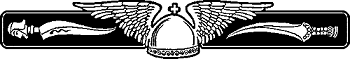
\includegraphics[width=9.3cm]{viking-tales/028}\\
    The Sea Fight}

\lettrine{M}{any} men felt as Solfi did. So when King Audbiorn and King
Arnvid sent out their war arrows, a great host gathered. All men came by
sea. Two hundred ships lay at anchor in the fiord, looking like strange
swimming animals because of their high carved prows and bright paint.
There were red and gold dragons with long necks and curved tails.
Sea-horses reared out of the water. Green and gold snakes coiled up.
Sea-hawks sat with spread wings ready to fly. And among all these curved
necks stood up the tall, straight masts with the long yardarms swinging
across them holding the looped-up sails.

When the starting horn blew, and their sails were let down, it was like
the spreading of hundreds of curious flags. Some were striped black and
yellow or blue and gold. Some were white with a black raven or a brown
bear embroidered on them, or blue with a white sea-hawk, or black with a
gold sun. Some were edged with fur. As the wind filled the gaudy sails,
and the ships moved off, the men waved their hands to the women on shore
and sang:

\begin{quote}
``To the sea! To the sea!\\
The wind in our sail,\\
The sea in our face,\\
And the smell of the fight.\\
After ship meets ship,\\
In the quarrel of swords\\
King Harald shall lie\\
In the caves under sea\\
And Norsemen shall laugh.''
\end{quote}

In the prow stood men leaning forward and sniffing the salt air with
joy. Some were talking of King Harald.

``Yesterday he had a hard fight,'' they said. ``To-day he will be lying
still, dressing his wounds and mending his ships. We shall take him by
surprise.''

They sailed near the coast. Solfi in his ``Sea-hawk'' was ahead leading
the way. Suddenly men saw his sail veer and his oars flash out. He had
quickly turned his boat and was rowing back. He came close to King
Arnvid and called:

``He is there, ahead. His boats are ready in line of battle. The fox has
not been asleep.''

King Arnvid blew his horn. Slowly his boats came into line with his
``Sea-stag'' in the middle. Again he blew his horn. Cables were thrown
across from one prow to the next, and all the ships were tied together
so that their sides touched. Then the men set their sails again and they
went past a tongue of land into a broad fiord. There lay the long line
of King Harald's ships with their fierce heads grinning and mocking at
the newcomers. Back of those prows was what looked like a long wall with
spots of green and red and blue and yellow and shining gold. It was the
locked shields of the men in the bows, and over every shield looked
fierce blue eyes. Higher up and farther back was another wall of
shields; for on the half deck in the stern of every ship stood the
captain with his shield-guard of a dozen men.

Arnvid's people had furled their sails and were taking down the masts,
but the ships were still drifting on with the wind. The horn blew, and
quickly every man sprang to his place in bow and stern. All were leaning
forward with clenched teeth and widespread nostrils. They were clutching
their naked swords in their hands. Their flashing eyes looked over their
shields.

Soon King Arnvid's ships crashed into Harald's line, and immediately the
men in the bows began to swing their swords at one another. The soldiers
of the shield-guard on the high decks began to throw darts and stones
and to shoot arrows into the ships opposite them.

So in every ship showers of stones and arrows were falling, and many men
died under them or got broken arms or legs. Spears were hurled from deck
to deck and many of them bit deep into men's bodies. In every bow men
slashed with their swords at the foes in the opposite ship. Some jumped
upon the gunwale to get nearer or hung from the prow-head. Some even
leaped into the enemy's boat.

King Harald's ship lay prow to prow with King Arnvid's. The battle had
been going on for an hour. King Harald was still in the stern on the
deck. There was a dent in his helmet where a great stone had struck.
There was a gash in his shoulder where a spear had cut. But he was still
fighting and laughed as he worked.

``Wolf meets wolf to-day,'' he said. ``But things are going badly in the
prow,'' he cried. ``Ivar fallen, Thorstein wounded, a dozen men lying in
the bottom of the boat!''

He leaped down from the deck and ran along the gunwale, shouting as he
went:

``Harald and victory!''

So he came to the bow and stood swinging his sword as fast as he
breathed. Every time it hit a man of Arnvid's men. Harald's own warriors
cheered, seeing him.

``Harald and victory!'' they shouted, and went to work again with good
heart.

Slowly King Arnvid's men fell back before Harald's biting sword. Then
Harald's men threw a great hook into that boat and pulled it alongside
and still pushed King Arnvid's people back.

``Come on! Follow me!'' cried Harald.

Then he leaped into King Arnvid's boat, and his warriors followed him.

``He comes like a mad wolf,'' King Arnvid's men said, and they turned
and ran back below the deck.

Then Arnvid himself leaped down and stood with his sword raised.

``Can this young Shockhead make cowards of you all?'' he cried.

But Harald's sword struck him, and he fell dead. Then a big, bloody
viking of King Arnvid leaped upon the edge of the ship and stood there.
He held his drinking-horn and his sword high in his hands.

``Ran\footnote{See note about Ran on page~\pageref{ran}.} and not you,
Shockhead, shall have them and me!'' he cried, and leaped laughing into
the water and was drowned.

Many other warriors chose the same death on that terrible day.

\begin{figure}
    \centering
    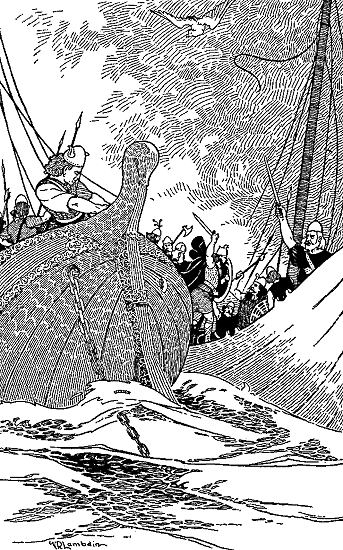
\includegraphics[width=9.1cm]{viking-tales/029}
    \caption{``Then he leaped into King Arnvid's boat''}
\end{figure}

All along the line of boats men fought for hours. In some places the
cables had been cut, and the boats had drifted apart. Ships lay
scattered about two by two, fighting. May boats sank, many men died,
some fled away in their ships, and at the end King Harald had won the
battle. So he had King Arnvid's country and King Audbiorn's country.
Many men took the oath and became his friends. All people were talking
of his wonderful battles.

\begin{figure}[hb]
    \centering
    \vskip8pt
    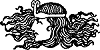
\includegraphics[width=2.7cm]{viking-tales/017}
\end{figure}
